\paragraph{Poisson-Nernst-Planck (PNP)}\label{subproject:PNP}
In this sub-project, the goal is to develop functionality for the detailed simulation of ionic dynamics in dendritic spines using the Poisson-Nernst-Planck system (``electro-diffusion''):
\begin{align}
  \frac{\partial c_{i}}{\partial t} \:& = \:  \nabla\cdot\left(D_{i}\nabla c_{i}+D_{i}
    \frac{z_{i}F}{RT}c_{i}\nabla\Phi\right) \label{eq:pnp_species}\\
  -\nabla(\varepsilon_{r}\varepsilon_{0}\nabla\Phi) \: & = \:
    \rho_{f}+\sum_{i}z_{i}Fc_{i} \label{eq:pnp_potential}
\end{align}
Equation (\ref{eq:pnp_species}) represents electro-diffusion for various ion species
$c_i$ with $D_i$ being diffusion coefficients; $z_i$ the ions' valencies; $F$, $R$
the Faraday and universal gas constants, respectively, and $T$ the temperature.
Equation (\ref{eq:pnp_potential}) is the Gauss law stating that the charged ions are
the sources for the electric field, represented by the negative gradient of the
electric potential $\Phi$. Here, $\varepsilon_r$, $\varepsilon_0$ are relative
permettivity and vacuum permettivity, resp.; $\rho_f$ is a fixed surface charge density.
\vspace{0.3cm}

The need for simulating ion movement, especially with regard to their
electrical properties, arises from the presence of charged filaments and membranes
throughout the neuron and notably at synapses. The effect of these charges on the
signal transduction and long-term development of neurons remains largely unclear.
Detailed simulations will shed light on the ion dynamics in domains on the micro-
and nano-scale present at, e.g., synaptic spines.

The agglomeration of ions at fixed surface charges is what makes this problem
computationally difficult: As equally charged ions are repelled and oppositely
charged ions are attracted, locally very steep concentration and with that:
very steep potential gradients form at these surfaces and the non-linear term
$c_{i}\nabla\Phi$ in equation (\ref{eq:pnp_species}) becomes very prominent,
making direct coupled solution of the system difficult.
\vspace{0.3cm}

Having run a first set of simulations on artificial dendritic spines with idealized longitudinal filaments inside the neck,
the next step will be to ascertain whether direction-specific effects can be
observed with differently oriented artificial filaments. In particular realistic
reconstructions of single spines and cells became recently
 available to this project which motivates using the realistic cell reconstructions
for simulations which aligns with another project initiated focusing on the
simulation of transcranial magnetic stimulation (TMS). Large-scale simulations
of TMS-induced calcium dynamics in spines and neurons using
the available cell reconstruction are planned. First proof-of-principle simulations
on the reconstruction, are shown in Fig.~\ref{fig:spine_simulation} (see Fig.~\ref{fig:spine} for an example of a spine geometry).

\begin{figure}[h!]
\centering
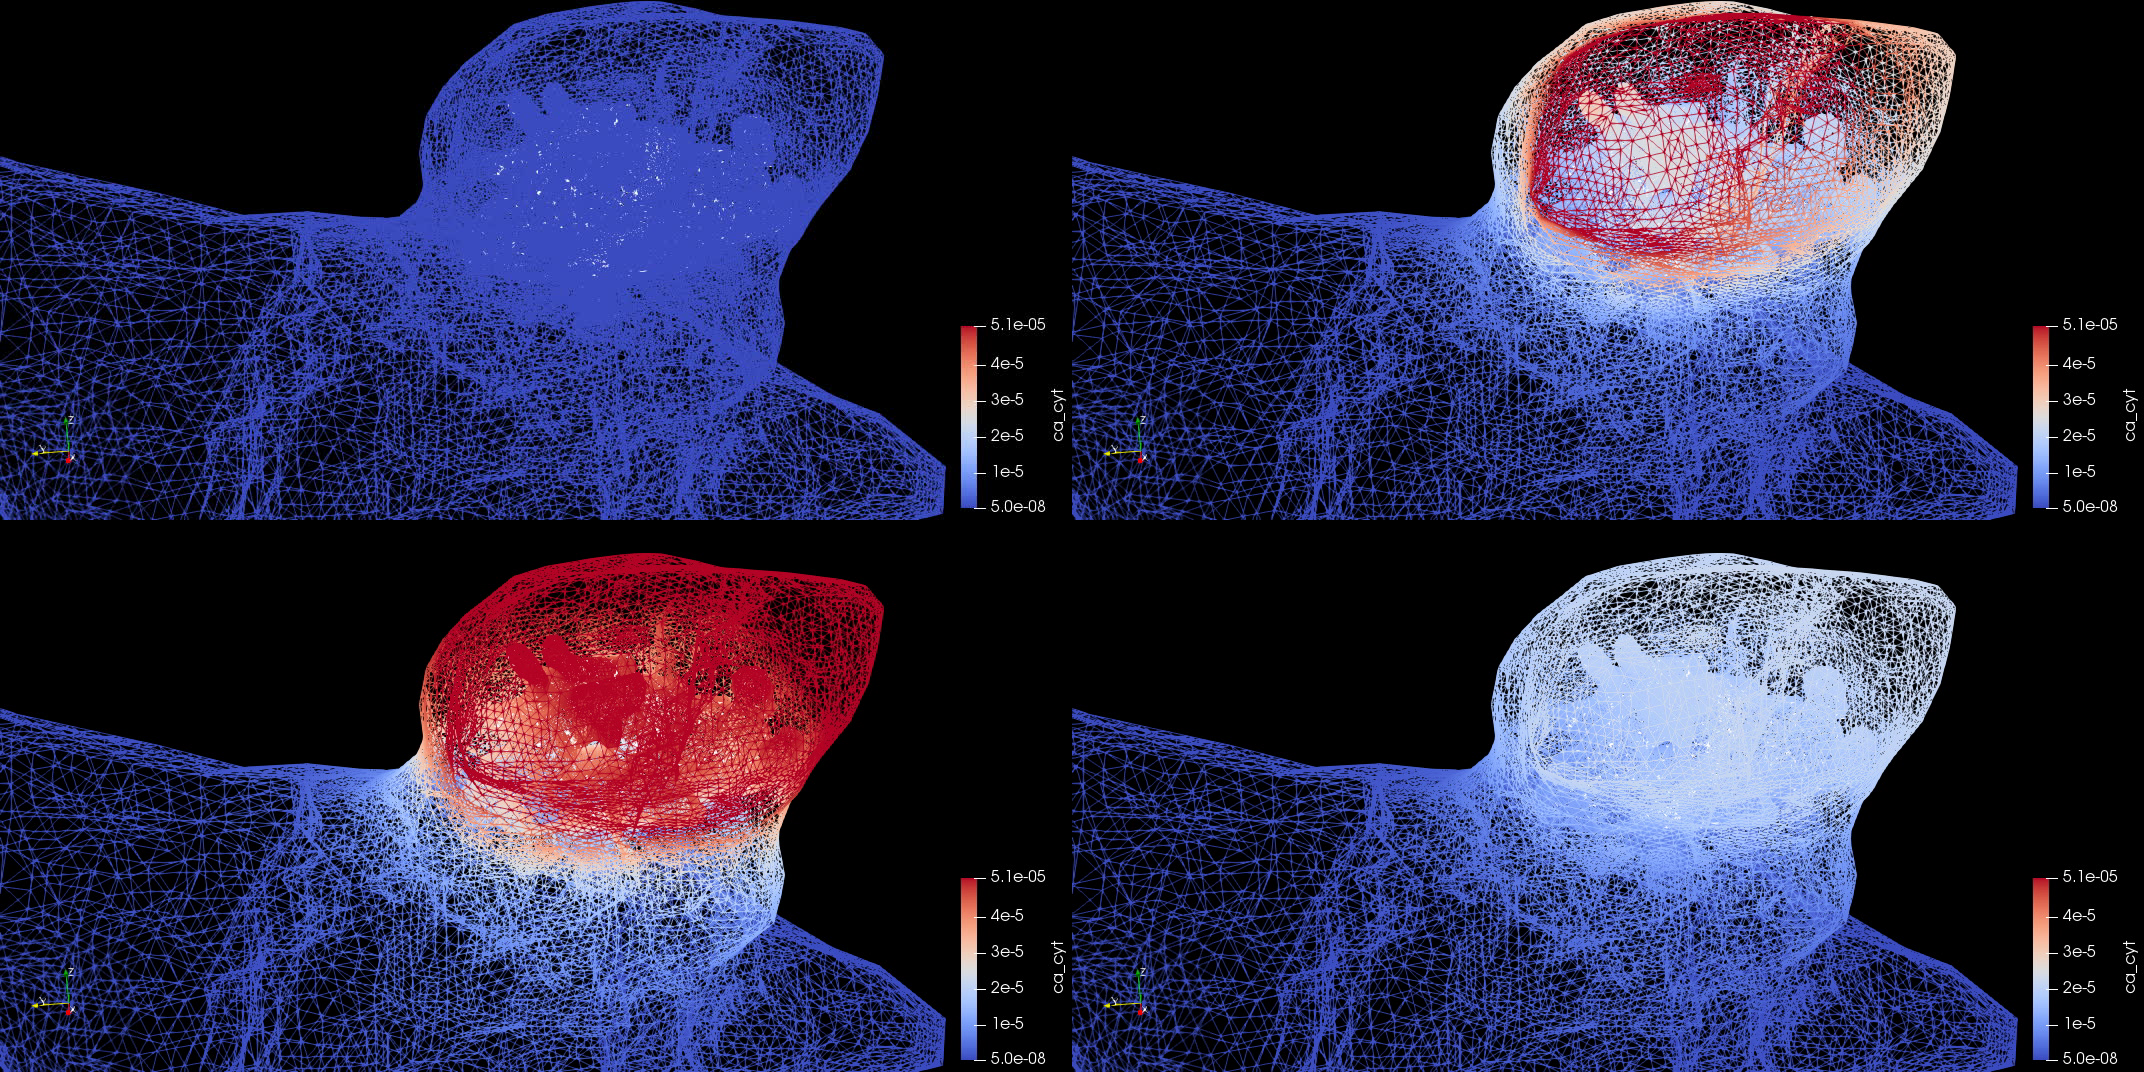
\includegraphics[scale=0.15]{inc/img/new_spine_simu.png}
\caption{\textbf{Simulation} run of the PNP model on a genuine reconstruction of a spine as displayed
in Fig. \ref{fig:spine}. Simulation time captured 10 ms, snapshots are taken (top left to bottom right) in 2.5 ms intervals.}
\label{fig:spine_simulation}
\end{figure}

\begin{figure}[h!]
\centering
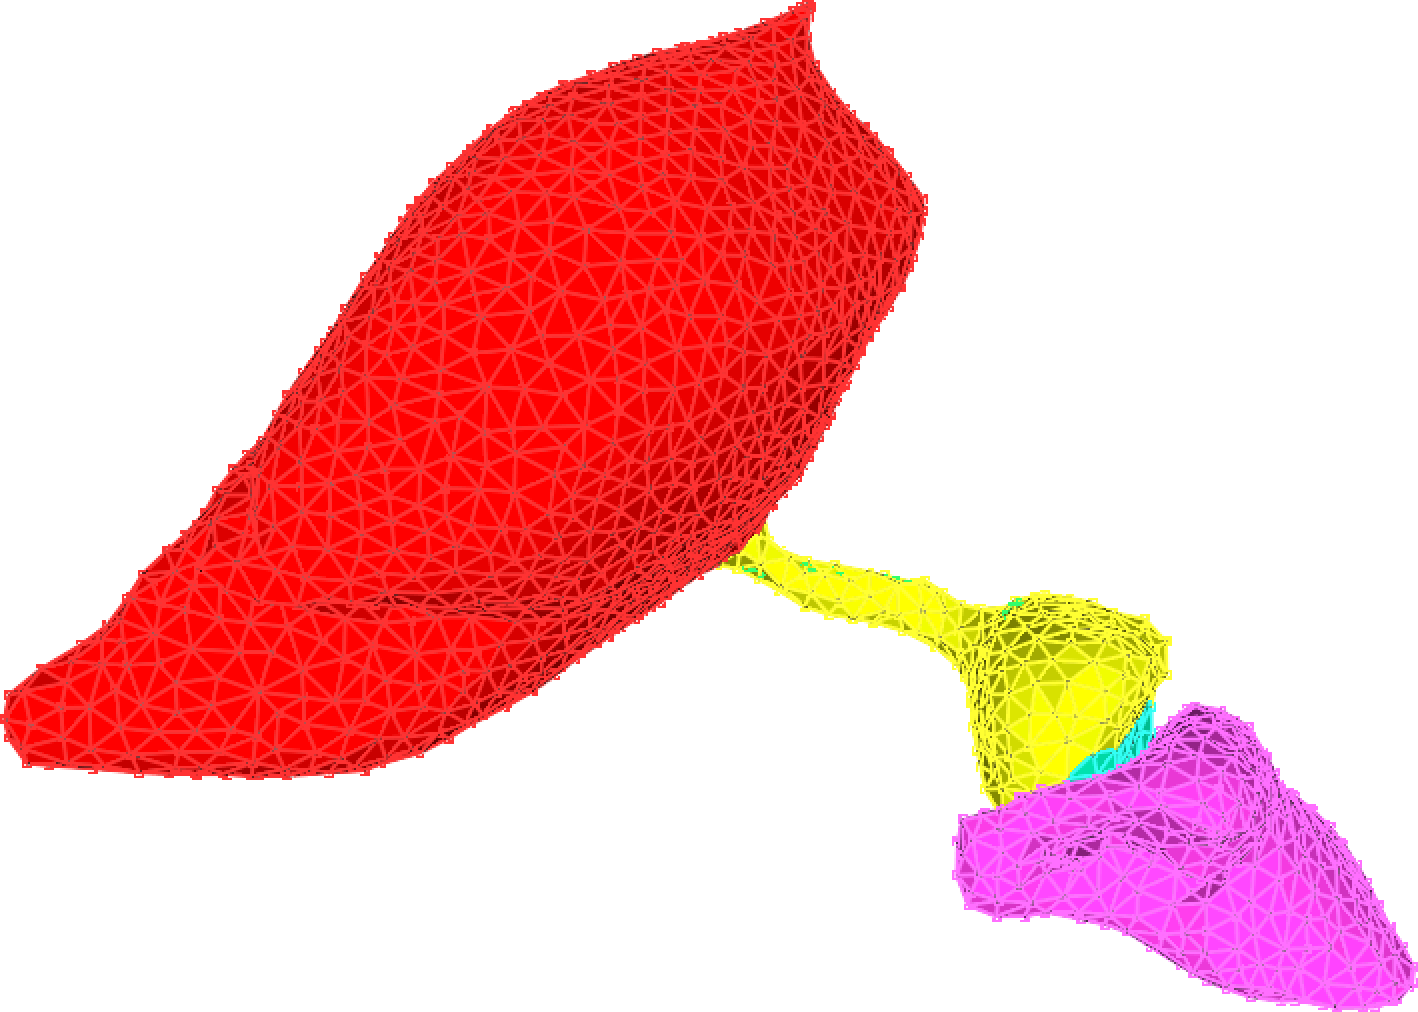
\includegraphics[scale=0.15]{inc/img/spine.png}
\caption{\textbf{Spine geometry}. Depicted is a human spine (yellow) reconstruction with
the common parts dendrite (red), presynapse (magenta), the post synaptic density (cyan)
and the endoplasmic reticulum hidden within the spine.}
\label{fig:spine}
\end{figure}

\noindent \textbf{Estimate of proposed simulation runs:} 48,080, divided into 48,000 runs of shorter 
length on SDSC Comet and and 80 longer runs on TACC Stampede2 for detailed simulations on the TMS project. 
Coarse grain simulation runs on reconstructed spines will be conducted on 10 spines in total.
Parameters to vary: Channel densities (6), boundary conditions (4), initial conditions (4),
each parameter is varied 20 times for parameter sweeps, totaling $10 \times 6 \times 10 \times 4
\times 20 = 48,000$ runs. Towards publication-level simulations, 20 spines will be analyzed with critical parameter sets (4) on high
resolution, thus totaling 80 runs on Stampede2. For a comprehensive overview of the parameter sets we refer to \cite{Breit2018b}.

\paragraph{Dimension-switching multigrid (DSMG)}
In this sub-project the calcium dynamics in a compartmentalized neuron will be modeled.
The endoplasmic reticulum (ER) is a multifunctional intracellular organelle of a neuron,
which consists of a complex three-dimensional network of connected endomembrane
tubules, stacks and cisternae, and is involved in various ion exchange processes,
%cf. Fig.~\ref{fig:schematics},
\cite{Breit2018}, ultimately responsible for synaptic plasticity, `cell within a cell'
structure, cf. \cite{Berridge1998}.

\begin{figure}
\centering
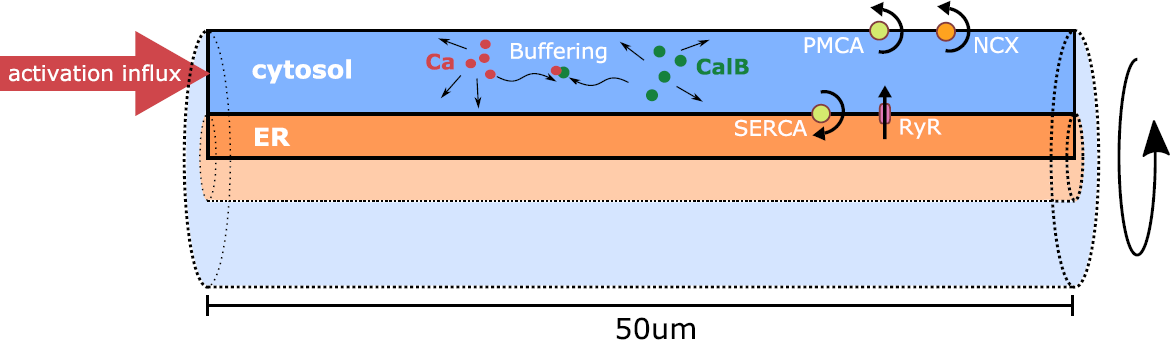
\includegraphics[scale=0.25]{inc/img/schematics.png}
\caption{\textbf{Model geometry}. Simulation domain and model components. The example domain is a cylindrical dendrite 50 $\mu$m in length with variable radius containing a centrally positioned cylindrical ER of variable radius. The rotational symmetry of the domain was used to reduce the problem to two dimensions (axial and radial position). The calcium model contains calcium in the cytosol and the ER as well as calbindin (CalB) in the cytosol. The dynamics of both are governed by a diffusive process and a buffering reaction. Calcium can cross the ER membrane through RyR channels and SERCA pumps, the plasma membrane through PMCA and NCX pumps.}
\label{fig:schematics}
\end{figure}

Of interest are the three-dimensional spatio-temporal $\textrm{Ca}^{2+}$ and $\textrm{IP}_3$ dynamics in the intracellular space of a neuron.
This is modeled by a system of diffusion-reaction equations described in the following.
The boundary conditions for this partial differential equation system are specifed by certain $\textrm{Ca}^{2+}$ and $\textrm{IP}_3$-dependent fluxes which depend on the chosen electrophysiogical stimulation protocol of the neuron.
Mobility in the neuron respectively ER is described by diffusion equations for the four quantities calcium (cytosolic ($c_c$) and endoplasmic ($c_e$)), calbindin-D28k ($b$), and $\textrm{IP}_3$ ($p$), which is required to model $\textrm{IP}_3$ receptors embedded in the endoplasmic membrane
\begin{equation}
\frac{\partial u}{\partial t} = \nabla \cdot (D \nabla u)
\end{equation}
where $u(x, t)$ stands for the four quantities mentioned above.
The diffusion constants $D$ are defined by data available in the literature \cite{Allbritton1992, Schmidt2003}.
The interaction between cytosolic $\textrm{Ca}^{2+}$ calbindin-$\textrm{D}_{28k}$ (CalB) is described by:
\begin{align}
  \mathrm{Ca}^{2+}+\mathrm{CalB}\;\xrightleftharpoons
  [\kappa_{b}^{-}]{\kappa_{b}^{+}}\;[\mathrm{CalBCa}^{2+}].
\end{align}

\noindent The full domain equations for cytosolic calcium and calbindin are thus given by
\begin{align}
  \delT{\ccyt} & \;=\; \nabla \cdot \left( D_{c} \nabla \ccyt \right) \;+\;
    \left(\kappa_{b}^{-}\left(b^{\mathrm{tot}}-b\right)
        -\kappa_{b}^{+}\:b\:\ccyt\right), \label{eq:ccyt}\\
  \delT{b} & \;=\; \nabla \cdot \left( D_{b} \nabla b \right) \;+\;
    \left(\kappa_{b}^{-}\left(b^{\mathrm{tot}}-b\right)
        -\kappa_{b}^{+}\:b\:\ccyt\right)  \label{eq:buff}
\end{align}

\noindent Exponential IP\textsubscript{3} decay towards a basal IP\textsubscript{3} concentration
$p^r$ in the cytosolic space is modeled by a reaction term that is added to the
IP\textsubscript{3} diffusion equation, leading to the diffusion-reaction equation
\begin{align}
  \delT{\ip3} & \;=\; D_p\Delta\ip3 \;-\; \kappa_{\ip3}\left(\ip3-{\ip3}^{r}\right)
\end{align}
for IP\textsubscript{3} in the cytosolic domain.
Endoplasmic Ca\textsuperscript{2+} dynamics are modeled by simple diffusion
\begin{align}
  \delT{\cer} & \;=\; D_{c}\Delta\cer
\end{align}
in the endoplasmic domain. For numerical simulations, the four equations are
discretized in space using a finite volumes method, \cite{Eymard2000}.
%Control volumes are constructed as a Voronoi-like dual tesselation of the original
%tetrahedral mesh by connecting the mid-points of edges, faces and volumes through planar facets.
%The equations above must hold for all control volumes, giving rise to one equation per control volume.
Time discretization is realized using a backwards Euler scheme. The described PDE problem
should be solved by a multigrid method, \cite{Brandt1977,Fedorenko1962,Hackbusch1976,Ruge1987}.
 If one designates with $\Omega_1$ the coarse domain and with $\Omega_2$ the fine
 domain and we require that the domains are nested, i. e. $\Omega_1 \subset \Omega_2$, and a restriction
operator $\mathcal{R}$ and a prolongation operator $\mathcal{P}$ exist one
can write the two grid iteration matrix by
\begin{equation}
u^{(i+1)} = G_2^{\nu_2}(Id - \mathcal{P}A_1^{-1}\mathcal{R}A_2)G_1^{\nu_1} u^{(i)} + \mathcal{P} A_1^{-1}\mathcal{R}f_2,
\end{equation}
where $Id$ is the identity matrix, $G_2$ a post smoothing matrix applied $\nu_2$ times, $G_1$ a pre smoothing matrix
applied $\nu_1$ times, $A_1$ and $A_2$ the matrices arising from the discretized PDE problem on the coarse respectively
fine domains $\Omega_1$ and $\Omega_2$ and $f_2$ the corresponding right hand side of the equation system arising by
discretization on the coarse domain $A_2 u_2 = f_2$. 

In traditional multigrid methods the restriction and prolongation operators are defined
between the same space dimension, i.e. information transfer from a coarse to a fine
grid level within the multigrid hierarchy. The \textbf{dimension-switching multigrid approach} 
we are developing will involve a new multigrid base level of reduced dimensionality, 
which will decrease computational cost. Some of the open topics are convergence rates and parallelization strategies.


\noindent \textbf{Estimate of proposed simulation runs:} 150 runs.
Approximately 50 shorter runs for development of the (parallel) correctness of the MPI program and to improve the parallel efficiency 
of the novel DSMG method and to demonstrate the scaling behaviour of the method will be required. 
Additionally the numerics of the newly developed DSMG algorithm needs to be compared to a standard
numerical problem, a time-dependent convection-diffusion equation on a reconstructed
neuron. To test for robustness of the numerical code 10 cells will be reconstructed,
5 simulation setups (boundary conditions and initial conditions will be varied around a reference case) 
will be run with the standard multigrid algorithm and 5 simulation setups will be run with the new
DSMG algorithm. Results of the runs each will be compared concerning convergence and precision
of the simulation result and contrasted with the results published in \cite{Breit2018}.

\paragraph{Network simulations of electrical and calcium dynamics (NET/CD)}
We have been been developing simulation techniques
for large-scale neuronal network simulations of networks described by graphs  (``1d'') with a
diameter information attached to the vertices (representing idealized, cylindrical or
cone-frustum compartments). The main results from this have been published in \cite{Breit2016}.
We have also developed functionality to couple these large-scale 1d network simulations to fully
resolved 3d reconstructed single-cell calcium simulations (similar to what is described in
\cite{Grein14}). In this kind of simulation, we aim to understand the functional role of calcium
as a messenger, taking into account the endoplasmic reticulum (ER) and a detailed model of the
calcium dynamics including buffers as well as important endoplasmic and plasma membrane calcium
exchange mechanisms such as the IP\textsubscript{3}R and RyR channels, voltage-dependent calcium
channels, and sarco-/endoplasmic reticulum or plasma membrane calcium ATP-ases \cite{Breit13, Breit2018a, Breit2018b}.
As the calcium dynamics are of special interest in the context of synaptic activity (e.g.,
synapse-to-nucleus communication), examining a single fully resolved cell within an active
network allows us to provide realistic synaptical inputs for the calcium simulation.
But even with rather artificial inputs (as, e.g., given by an experimental stimulation protocol),
single-cell calcium simulations and high-detail simulations of small regions of interest (as the
vicinity of one or more dendritic spines) have become more and more important in our ongoing work.

We would like to bring many aspects of the previous work together:
The goal is to investigate whole-cell calcium dynamics on the basis of realistic synaptic input
and membrane potential data from the 1d network model. In view of our basic parameter study
about the influence of geometric parameters on calcium wave elicitation, we want to assess
whether and under which circumstances calcium waves can occur within neurons in an active network:
Which synaptic input patterns can lead to such waves? Can a single firing synapse cause a calcium
signal cascade to the soma? Is the position of the synapse important (because of the
location-specific geometry of the dendrites and ER)? Or are action potentials the only way to
cause calcium influx into the soma (via voltage-dependent calcium channels)?
What is the role of back-propagating action potentials? Do they significantly affect the local
(synaptic) or even global calcium levels?
Investigating these kinds of questions in simulations has been a long-standing goal of our
research with implications for learning and cell survival. In past efforts a grid generation pipeline was developed with the
goal in mind to reconstruct arbitrary cells from the \textit{Neuromorpho.org} database \cite{Ascoli2007}
for the DMSG project and create a multigrid hiearchy. Existing tools, cf. \cite{Moerschel2017}, generated base levels too
fine grained and thus not suitable for HPC solvers. A new ansatz was made by
using spline data and grid generation tools from \ug which use point-diameter data.
Volume meshes are generated efficiently by grid generation algorithms for constrained
Delaunay triangulation \cite{Shewchuk2002, Si2005}. Based on these recent advances
this sub-project aims to investigate by systematic parameter studies the calcium
dynamics using the PNP model in the reconstructed cells on the sub-cellular level.

\noindent \textbf{Estimate of proposed simulation runs:} 1010 runs.
During development some performance bottlenecks where introduced by design of simplicity in the 1d/3d coupling method.
For optimization and increasing the fraction of parallel code and thus to improve scaling
approximately 10 runs will be needed to vary parts of the algorithm for benchmarking
and optimization. An average neuron in the Neocortex has roughly 1000 synapses,
 cf. \cite{Drachman2004}. 1000 runs (Synapse location will be varied)
for production will be used to assess if a \textit{single} firing synapse can cause a signal cascade up to the soma. 

\begin{figure}[!h]
\centering
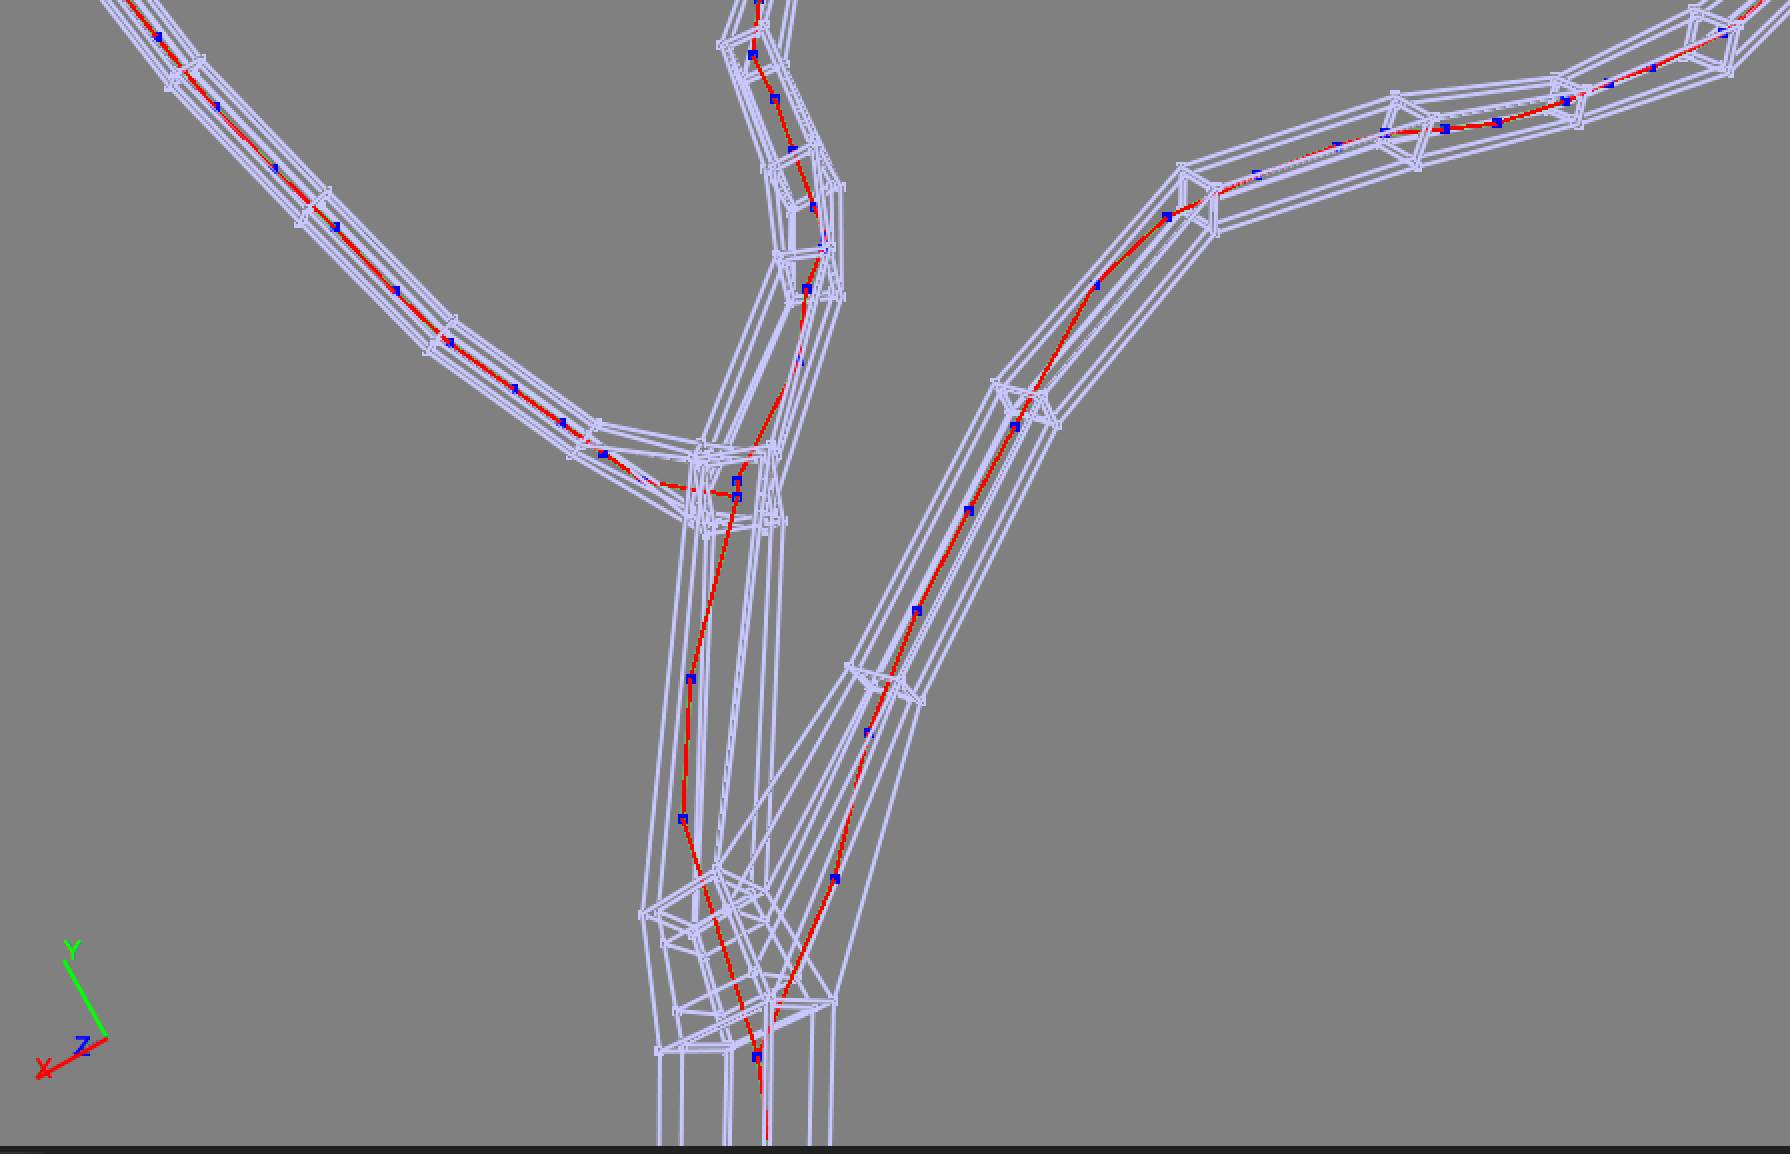
\includegraphics[scale=0.20]{inc/img/mesh.png}
\caption{\textbf{Grid hierarchy} which shows a neuron with ER on the base level
 (wireframe mesh) and the new coarse level (1d line segments).}
\label{fig:base_level}
\end{figure}

Resources will be used for testing new methods and for running production code. All participants in the project will have access to a shared file in which an estimated demand for compute time for the following project month can be submitted. Stephan Grein will coordinate the internal distribution of compute time for the subsequent month by weighing the individual demand against mile stone deadlines, demand for conference contributions, theses finalizations and other constraint parameters. Through this method, contingent overflow as well as monthly over-demand can be minimized. A preliminary year schedule is provided below in the Ganttchart.

\begin{ganttchart}[vgrid, hgrid, bar/.style={fill=blue!50},
                    y unit chart = 0.4cm, y unit title = 0.4cm, title height=1,
                    bar height=0.4]{1}{12}
  \scriptsize
  \gantttitle{Project Month}{12} \\
  \gantttitlelist{1,...,12}{1} \\
  \ganttgroup{\textbf{PNP}}{1}{12} \\
    \ganttbar[bar/.style={fill=red}]{\scriptsize electro-diffusion through reconstructed patches}{1}{6}\\
    \ganttbar[bar/.style={fill=red}]{\scriptsize TMS simulations on reconstructed spines}{7}{12} \\
  \ganttgroup{\textbf{DMSG}}{1}{12} \\
    \ganttbar[bar/.style={fill=red}]{\scriptsize develop grid generation methods}{1}{3}\\
    \ganttbar[bar/.style={fill=red}]{\scriptsize develop dimension-switching multigrid (MG) methods}{4}{9}\\
    \ganttbar[bar/.style={fill=red}]{\scriptsize bechmark dimension-switching MG and conduct parameter study}{9}{12} \\
  \ganttgroup{\textbf{NET/CD}}{1}{12} \\
    \ganttbar[bar/.style={fill=red}]{\scriptsize large-scale whole-cell simulations}{1}{9} \\
    \ganttbar[bar/.style={fill=red}]{\scriptsize calcium waves in coupled network/whole-cell simulations}{1}{8} \\
    \ganttbar[bar/.style={fill=red}]{\scriptsize back-propagating APs in 1d/3d coupled simulations}{10}{12} \\
    \ganttbar[bar/.style={fill=red}]{\scriptsize systematic TMS simulations on networks/whole-cell}{10}{12} 
\end{ganttchart}

Numerical experiments will be designed by the PI and Stephan Grein, setup, submissions 
to the cluster and data analyis of the results is conducted by Stephan Grein.

\paragraph{PNP}
Examine the electro-diffusion properties through reconstructed pathes of actin and filament networks. 
Examine TMS simulations on detailed anatomical reconstructions of dendritic spines.

\paragraph{DSGM}
Develop and benchmark grid generation with refinement projectors, develop the dimension-switching multigrid operators and benchmark and conduct parameter study of the surrogate
neurobiological problem.

\paragraph{NET/CD}
Large-scale whole-cell simulations of \textit{Neuromorpho.org} \cite{Ascoli2007} database.
Investigating calcium waves in coupled network/whole-cell simulations, back-propagating
action potentials in 1d/3d coupled simulations and systematic TMS simulations on networks/whole-cell
